\part{HTML5}


\chapter{Introduction}

HTML5 is a markup language used for structuring and presenting content for the World Wide Web and a core technology of the Internet. It is the fifth revision of the HTML standard (created in 1990 and standardized as HTML 4 as of 1997) and, as of December 2012, is a candidate recommendation of the World Wide Web Consortium (W3C). Its core aims have been to improve the language with support for the latest multimedia while keeping it easily readable by humans and consistently understood by computers and devices (web browsers, parsers, etc.). HTML5 is intended to subsume not only HTML 4, but also XHTML 1 and DOM Level 2 HTML.

HTML 5 是下一代的 HTML,现在仍处于完善之中,但是大部分现代浏览器已经具备了某些 HTML5 支持。

Following its immediate predecessors HTML 4.01 and XHTML 1.1, HTML5 is a response to the fact that the HTML and XHTML in common use on the World Wide Web are a mixture of features introduced by various specifications, along with those introduced by software products such as web browsers, those established by common practice, and the many syntax errors in existing web documents. It is also an attempt to define a single markup language that can be written in either HTML or XHTML syntax. It includes detailed processing models to encourage more interoperable implementations; it extends, improves and rationalises the markup available for documents, and introduces markup and application programming interfaces (APIs) for complex web applications. For the same reasons, HTML5 is also a potential candidate for cross-platform mobile applications. Many features of HTML5 have been built with the consideration of being able to run on low-powered devices such as smartphones and tablets. In December 2011, research firm Strategy Analytics forecast sales of HTML5 compatible phones will top 1 billion in 2013.

In particular, HTML5 adds many new syntactic features. These include the new <video>, <audio> and <canvas> elements, as well as the integration of scalable vector graphics (SVG) content (that replaces the uses of generic <object> tags) and MathML for mathematical formulas. These features are designed to make it easy to include and handle multimedia and graphical content on the web without having to resort to proprietary plugins and APIs. Other new elements, such as <section>, <article>, <header> and <nav>, are designed to enrich the semantic content of documents. New attributes have been introduced for the same purpose, while some elements and attributes have been removed. Some elements, such as <a>, <cite> and <menu> have been changed, redefined or standardized. The APIs and Document Object Model (DOM) are no longer afterthoughts, but are fundamental parts of the HTML5 specification.[5] HTML5 also defines in some detail the required processing for invalid documents so that syntax errors will be treated uniformly by all conforming browsers and other user agents.

\chapter{History}

The Web Hypertext Application Technology Working Group (WHATWG) began work on the new standard in 2004. At that time, HTML 4.01 had not been updated since 2000, and the World Wide Web Consortium (W3C) was focusing future developments on XHTML 2.0. In 2009, the W3C allowed the XHTML 2.0 Working Group's charter to expire and decided not to renew it. W3C and WHATWG are currently working together on the development of HTML5.

While HTML5 is often compared to Flash, the two technologies are very different. Both include features for playing audio and video within web pages, and for using Scalable Vector Graphics. HTML5 on its own cannot be used for animation and interactivity — it must be supplemented with CSS3 or JavaScript. There are many Flash capabilities that have no direct counterpart in HTML5. 

Although HTML5 has been well known among web developers for years, it became the topic of mainstream media around April 2010 after Apple Inc's then-CEO Steve Jobs issued a public letter titled "Thoughts on Flash" where he concludes that "[Adobe] Flash is no longer necessary to watch video or consume any kind of web content" and that "new open standards created in the mobile era, such as HTML5, will win". This sparked a debate in web development circles where some suggested that while HTML5 provides enhanced functionality, developers must consider the varying browser support of the different parts of the standard as well as other functionality differences between HTML5 and Flash. In early November 2011, Adobe announced that it will discontinue development of Flash for mobile devices and reorient its efforts in developing tools utilizing HTML5.


\section{Standardization process}

The Mozilla Foundation and Opera Software presented a position paper at a World Wide Web Consortium (W3C) workshop in June 2004, focusing on developing technologies that are backward compatible with existing browsers,[18] including an initial draft specification of Web Forms 2.0. The workshop concluded with a vote, 8 for, 14 against, for continuing work on HTML. Later that month, work based upon that position paper moved to the newly formed Web Hypertext Application Technology Working Group (WHATWG), and a second draft, Web Applications 1.0, was also announced. The two specifications were later merged to form HTML5. The HTML5 specification was adopted as the starting point of the work of the new HTML working group of the W3C in 2007.

\begin{compactitem}
\item 2008 – First Public Working Draft

WHATWG published the First Public Working Draft of the specification on 22 January 2008.[22] Parts of HTML5 have been implemented in browsers despite the whole specification not yet having reached final Recommendation status.

\item 2011 – Last Call

On 14 February 2011, the W3C extended the charter of its HTML Working Group with clear milestones for HTML5. In May 2011, the working group advanced HTML5 to "Last Call", an invitation to communities inside and outside W3C to confirm the technical soundness of the specification. The W3C is developing a comprehensive test suite to achieve broad interoperability for the full specification by 2014, which is now the target date for Recommendation.[23] In January 2011, the WHATWG renamed its "HTML5" living standard to "HTML". The W3C nevertheless continues its project to release HTML5.

\item 2012 – Candidate Recommendation

In July 2012, WHATWG and W3C decided on a degree of separation. W3C will continue the HTML5 specification work, focusing on a single definitive standard, which is considered as a "snapshot" by WHATWG. The WHATWG organization will continue its work with HTML5 as a "Living Standard". The concept of a living standard is that it is never complete and is always being updated and improved. New features can be added but functionality will not be removed.

In December 2012, W3C designated HTML5 as a Candidate Recommendation. The criterion for advancement to W3C Recommendation is "two 100\% complete and fully interoperable implementations".

\end{compactitem}





\section{Plan 2014}

In September 2012, the W3C proposed a plan to release a stable HTML5 Recommendation by the end of 2014 and an HTML 5.1 specification Recommendation by the end of 2016.

\subsection{Core HTML specification}

The combined timelines for HTML 5.0, HTML 5.1 and HTML 5.2:

\begin{table}[!h]
\centering
\begin{tabular}{|l|l|l|l|l|l|}
\hline
		& 2012			& 2013			& 2014			& 2015			& 2016	\\
\hline
HTML 5.0& Candidate Rec	& Call for Review	& Recommendation	& 				& 		\\
\hline
HTML 5.1& 1st Working Draft&				& Last Call		& Candidate Rec	& Recommendation	\\
\hline
HTML 5.2& 				&				& 				& 1st Working Draft &				\\
\hline
\end{tabular}
\end{table}

The W3C proposed a greater reliance on modularity as a key part of the plan to make faster progress, meaning identifying specific features, either proposed or already existing in the spec, and advancing them as separate specifications. Some technologies that were originally defined in HTML5 itself are now defined in separate specifications:

\begin{compactitem}
\item HTML Working Group – Microdata, HTML Canvas 2D Context
\item Web Apps WG – Web Messaging, Web Workers, Web Storage, WebSocket API, Server-Sent Events
\item IETF HyBi WG – WebSocket Protocol
\item WebRTC WG – WebRTC
\item W3C Web Media Text Tracks CG – WebVTT
\end{compactitem}

Some specifications that were initially developed standalone have been adapted as HTML5 extensions or features by reference: SVG, MathML, WAI-ARIA.

\begin{figure}[!h]
\centering
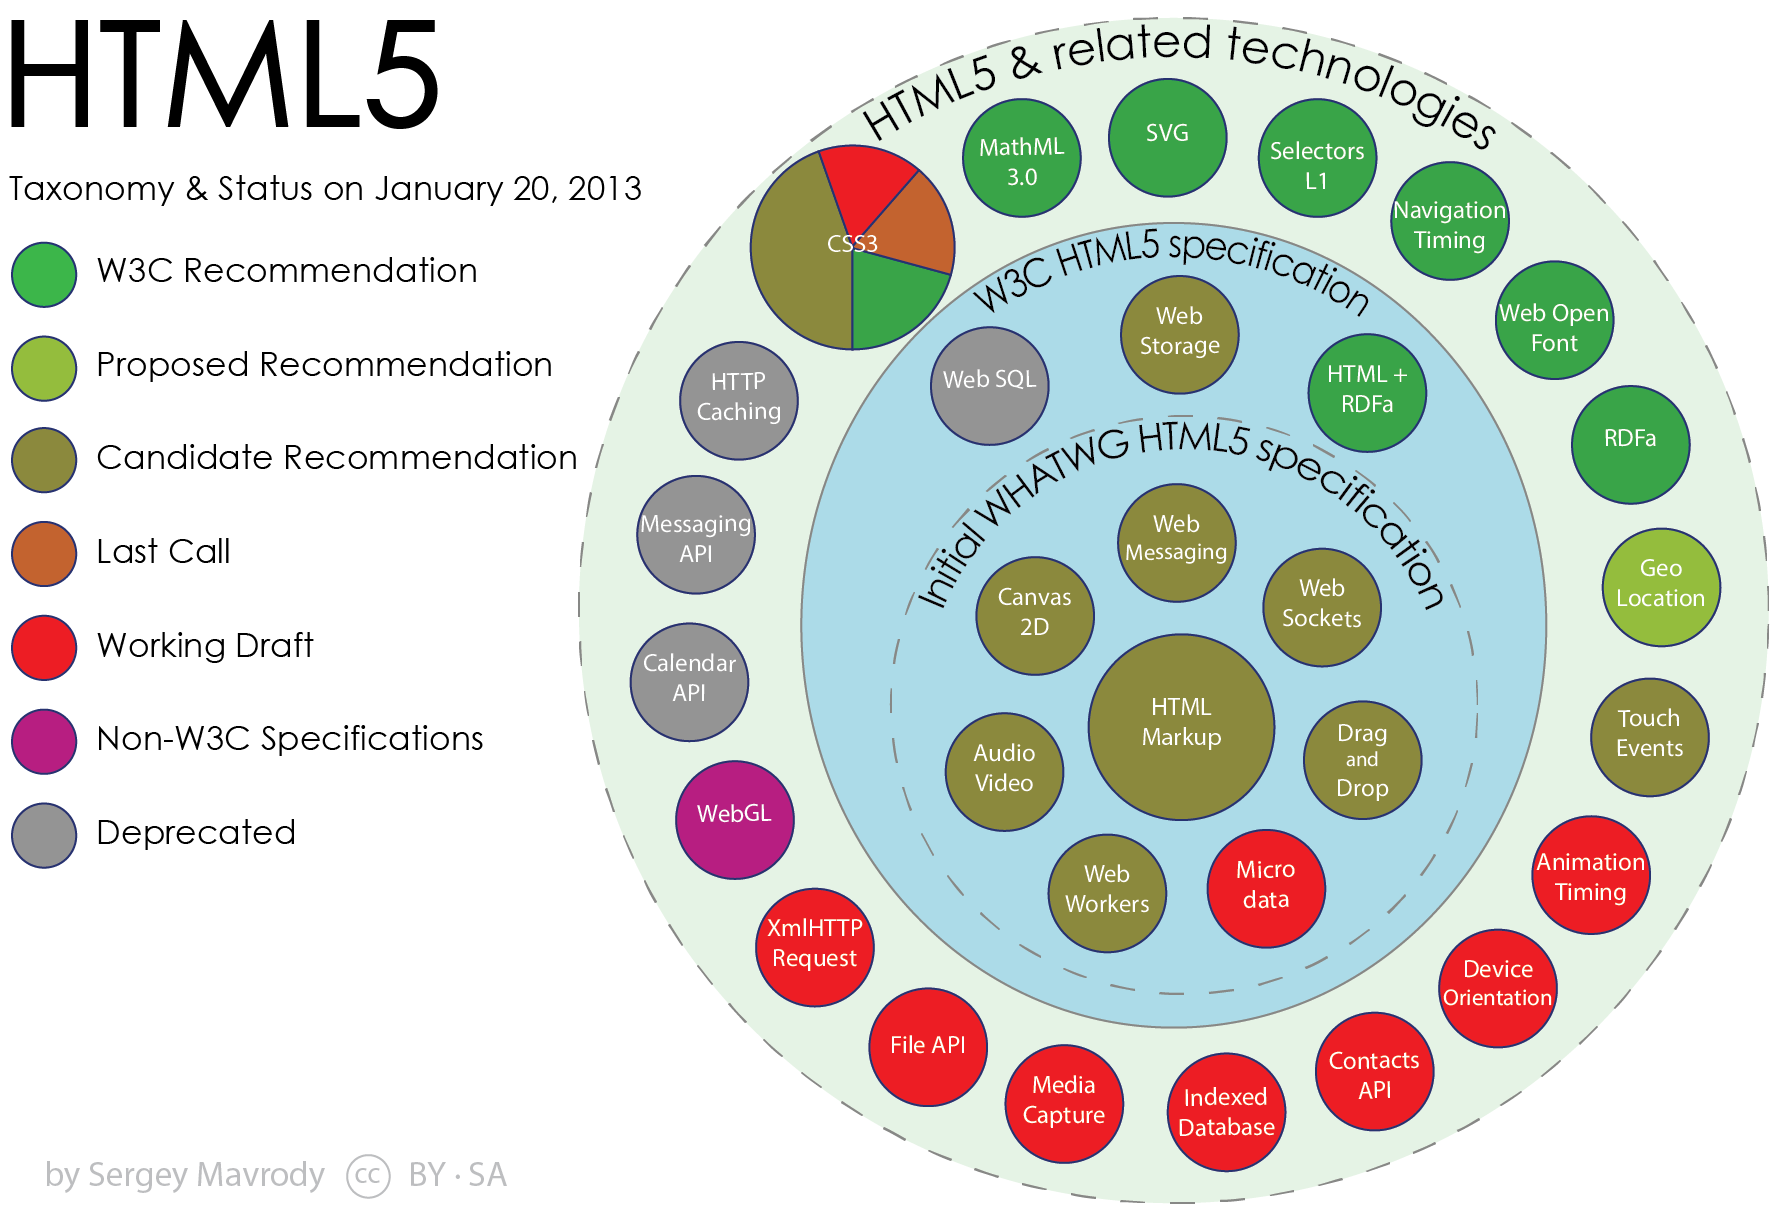
\includegraphics[scale=0.2]{HTML5-APIs-and-related-technologies.png}
\caption{HTML5 APIs and related technologies}
\label{HTML5-APIs-and-related-technologies}
\end{figure}

\chapter{Features}




\section{Markup}


HTML5 introduces elements and attributes that reflect typical usage on modern websites. Some of them are semantic replacements for common uses of generic block (<div>) and inline (<span>) elements, for example <nav> (website navigation block), <footer> (usually referring to bottom of web page or to last lines of HTML code), or <audio> and <video> instead of <object>. Some deprecated elements from HTML 4.01 have been dropped, including purely presentational elements such as <font> and <center>, whose effects have long been superseded by the more capable Cascading Style Sheets. There is also a renewed emphasis on the importance of DOM scripting (e.g., JavaScript) in Web behavior.

The HTML5 syntax is no longer based on SGML despite the similarity of its markup. It has, however, been designed to be backward compatible with common parsing of older versions of HTML. It comes with a new introductory line that looks like an SGML document type declaration, <!DOCTYPE html>, which triggers the standards-compliant rendering mode. As of 5 January 2009, HTML5 also includes Web Forms 2.0, a previously separate WHATWG specification.



\section{APIs}


In addition to specifying markup, HTML5 specifies scripting application programming interfaces (APIs) that can be used with JavaScript. Existing document object model (DOM) interfaces are extended and de facto features documented. There are also new APIs, such as:

\begin{compactitem}
\item The canvas element for immediate mode 2D drawing. See Canvas 2D API Specification 1.0 specification
\item Timed media playback
\item Offline Web Applications[39]
\item Document editing
\item Drag-and-drop
\item Cross-document messaging
\item Browser history management
\item MIME type and protocol handler registration
\item Microdata
\item Web Storage, a key-value pair storage framework that provides behaviour similar to cookies but with larger storage capacity and improved API
\end{compactitem}


Not all of the above technologies are included in the W3C HTML5 specification, though they are in the WHATWG HTML specification. Some related technologies, which are not part of either the W3C HTML5 or the WHATWG HTML specification, are as follows. The W3C publishes specifications for these separately:

\begin{compactitem}
\item Geolocation
\item Web SQL Database, a local SQL Database (no longer maintained).
\item The Indexed Database API, an indexed hierarchical key-value store (formerly WebSimpleDB).
\item HTML5 File API, handles file uploads and file manipulation.
\item Directories and System, an API intended to satisfy client-side-storage use cases not well served by databases.
\item File Writer, an API for writing to files from web applications.
\item Web Audio API, a high-level JavaScript API for processing and synthesizing audio in web applications.
\end{compactitem}

HTML5 alone cannot provide animation within web pages. Either JavaScript or CSS3 is necessary for animating HTML elements. Animation is also possible using JavaScript and HTML 4, and within SVG elements through SMIL, although browser support of the latter remains uneven as of 2011.



\section{XHTML5}


XHTML5 is the XML serialization of HTML5. XML documents must be served with an XML Internet media type (often confused with MIME type) such as application/xhtml+xml or application/xml. XHTML5 requires XML's strict, well-formed syntax. The choice between HTML5 and XHTML5 boils down to the choice of a MIME/content type: the media type one chooses determines what type of document should be used. In XHTML5, the HTML5 doctype html is optional and may simply be omitted. HTML that has been written to conform to both the HTML and XHTML specifications—and which will therefore produce the same DOM tree whether parsed as HTML or XML—is termed "polyglot markup".



\section{Error handling}

HTML5 is designed so that old browsers can safely ignore new HTML5 constructs.[citation needed] In contrast to HTML 4.01, the HTML5 specification gives detailed rules for lexing and parsing, with the intent that different compliant browsers will produce the same result in the case of incorrect syntax. Although HTML5 now defines a consistent behavior for "tag soup" documents, those documents are not regarded as conforming to the HTML5 standard.


\section{Popularity}

According to a report released on 30 September 2011, 34 of the world's top 100 Web sites were using HTML5 – the adoption led by search engines and social networks. Another report released in July 2013 has shown that 153 of the Fortune 500 U.S. companies already implemented HTML5 on their corporate websites.



\section{Difference frome HTML 4.01 and XHTML 1.x}


The following is a cursory list of differences and some specific examples.

\begin{compactitem}
\item New parsing rules: oriented towards flexible parsing and compatibility; not based on SGML
\item Ability to use inline SVG and MathML in text/html
\item New elements: article, aside, audio, bdi, canvas, command, data, datalist, details, embed, figcaption, figure, footer, header, keygen, mark, meter, nav, output, progress, rp, rt, ruby, section, source, summary, time, track, video, wbr
\item New types of form controls: dates and times, email, url, search, number, range, tel, color
\item New attributes: charset (on meta), async (on script)
\item Global attributes (that can be applied for every element): id, tabindex, hidden, data-* (custom data attributes)
\item Deprecated elements will be dropped altogether: acronym, applet, basefont, big, center, dir, font, frame, frameset, isindex, noframes, strike, tt
\end{compactitem}

dev.w3.org provides the latest Editors Draft of "HTML5 differences from HTML 4", which provides a complete outline of additions, removals and changes between HTML5 and HTML 4.



\chapter{Digital Rights Manage}


Industrial players including the BBC, Google, Microsoft, and Netflix have been lobbying for the inclusion of Encrypted Media Extensions (EME), a form of Digital Rights Management (DRM), into the HTML5 standard. As of the end of 2012 and the beginning of 2013, 27 organisations including the Free Software Foundation have started a campaign against including Digital Rights Management in the HTML5 standard. However in late September 2013, the W3C HTML working group decided that Encrypted Media Extensions, a form of DRM was "in scope" and will potentially be included in the HTML 5.1 standard






\chapter{Reconstruction use HTML5}












































